% =============================================================================
% CHAPITRE 1 - CINÉMATIQUE
% Partie 10 : Cinématique de rotation
% Version maritime pour l'IMQ
% =============================================================================

% =============================================================================
\section{Cinématique de rotation}
% =============================================================================

Jusqu'à présent, nous avons étudié le mouvement de \textbf{translation} : le déplacement d'un objet d'un point à un autre. Nous allons maintenant étudier le mouvement de \textbf{rotation} : le mouvement d'un objet qui tourne autour d'un axe fixe.

\begin{remarque}[title=La rotation dans le contexte maritime]
La rotation est omniprésente en navigation :
\begin{itemize}
    \item L'\textbf{hélice} qui propulse le navire
    \item Le \textbf{treuil} qui enroule les câbles
    \item Le \textbf{gouvernail} qui pivote pour diriger le navire
    \item Le \textbf{radar} qui effectue des balayages rotatifs
    \item Le \textbf{cabestan} pour les man\oe{}uvres d'amarrage
\end{itemize}
\end{remarque}

\subsection{Position angulaire et déplacement angulaire}

\begin{definition}[title=Position angulaire]
La \textbf{position angulaire} $\theta$ d'un objet en rotation est l'angle entre une ligne de référence fixe et une ligne tracée de l'axe de rotation jusqu'à l'objet.

L'unité SI de la position angulaire est le \textbf{radian} (rad).
\end{definition}

\begin{center}
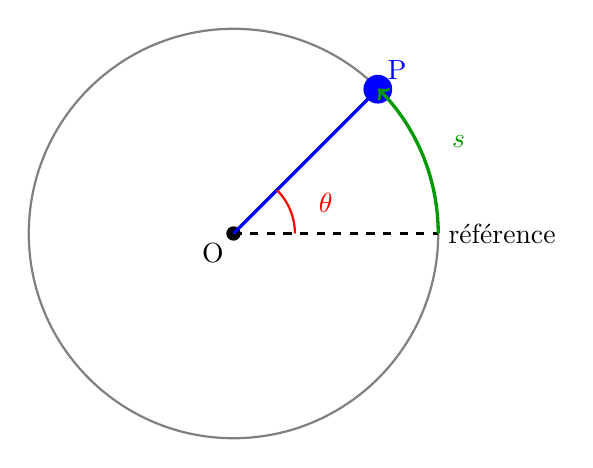
\begin{tikzpicture}[scale=1.3]
% Cercle
\draw[thick, gray] (0,0) circle (2);
% Axe de rotation
\fill (0,0) circle (2pt) node[below left] {O};
% Position initiale
\draw[thick, dashed] (0,0) -- (2,0) node[right] {référence};
% Position actuelle
\draw[very thick, blue] (0,0) -- (1.41,1.41);
\fill[blue] (1.41,1.41) circle (4pt) node[above right] {P};
% Angle
\draw[thick, red] (0.6,0) arc (0:45:0.6);
\node[red] at (0.9,0.3) {$\theta$};
% Arc
\draw[very thick, green!60!black, ->] (2,0) arc (0:45:2);
\node[green!60!black] at (2.2,0.9) {$s$};
\end{tikzpicture}
\end{center}

\subsubsection{Le radian}

Le \textbf{radian} est défini comme le rapport entre la longueur de l'arc $s$ et le rayon $r$ :

\begin{equationimportante}
\begin{equation}
\theta = \frac{s}{r} \quad \text{(en radians)}
\end{equation}
\end{equationimportante}

Un angle de 1 radian correspond à un arc de longueur égale au rayon.

\begin{center}
\renewcommand{\arraystretch}{1.4}
\begin{tabular}{|c|c|c|}
\hline
\rowcolor{bleuclair}
\textbf{Degrés} & \textbf{Radians} & \textbf{Tours} \\
\hline
$360°$ & $2\pi$ rad & 1 tour \\
\hline
$180°$ & $\pi$ rad & $\frac{1}{2}$ tour \\
\hline
$90°$ & $\frac{\pi}{2}$ rad & $\frac{1}{4}$ tour \\
\hline
$60°$ & $\frac{\pi}{3}$ rad & $\frac{1}{6}$ tour \\
\hline
$45°$ & $\frac{\pi}{4}$ rad & $\frac{1}{8}$ tour \\
\hline
$1°$ & $\frac{\pi}{180}$ rad $\approx 0,0175$ rad & -- \\
\hline
$57,3°$ & $1$ rad & -- \\
\hline
\end{tabular}
\end{center}

\begin{remarque}[title=Conversions]
\begin{align*}
\text{Degrés} \to \text{Radians} : \quad \theta_{rad} &= \theta_{deg} \times \frac{\pi}{180} \\[0.3cm]
\text{Radians} \to \text{Degrés} : \quad \theta_{deg} &= \theta_{rad} \times \frac{180}{\pi}
\end{align*}
\end{remarque}

\begin{definition}[title=Déplacement angulaire]
Le \textbf{déplacement angulaire} $\Delta\theta$ est la variation de la position angulaire :
\begin{equation}
\Delta\theta = \theta_f - \theta_i
\end{equation}

Convention de signes :
\begin{itemize}
    \item $\Delta\theta > 0$ : rotation dans le sens \textbf{antihoraire} (sens trigonométrique)
    \item $\Delta\theta < 0$ : rotation dans le sens \textbf{horaire}
\end{itemize}
\end{definition}

\subsection{Relation entre grandeurs linéaires et angulaires}

Pour un objet en rotation à une distance $r$ de l'axe, la longueur d'arc parcourue est reliée au déplacement angulaire :

\begin{equationimportante}
\begin{equation}
s = r\theta \quad \text{($\theta$ en radians)}
\end{equation}
\end{equationimportante}

\begin{exemple}{Câble enroulé sur un treuil}{}
Un treuil de rayon $\SI{15}{cm}$ effectue 5 tours complets. Quelle longueur de câble est enroulée?

\textbf{Déplacement angulaire :}
\[ \Delta\theta = 5 \text{ tours} \times 2\pi = 10\pi \text{ rad} \]

\textbf{Longueur de câble :}
\[ s = r\Delta\theta = 0,15 \times 10\pi = \SI{4,71}{m} \]
\end{exemple}

\begin{pratiqueautonome}
Un cabestan de rayon $\SI{20}{cm}$ effectue 8 tours complets pour haler un câble d'amarrage.

\begin{enumerate}[label=\alph*)]
    \item Quel est le déplacement angulaire en radians?
    \item Quelle longueur de câble a été halée?
\end{enumerate}

\espaceresolution[5cm]
\reponsepratique{a) $\Delta\theta = 16\pi \approx \SI{50,3}{rad}$ \quad b) $s \approx \SI{10,1}{m}$}
\end{pratiqueautonome}

\subsection{Vitesse angulaire}

\begin{definition}[title=Vitesse angulaire moyenne]
La \textbf{vitesse angulaire moyenne} $\omega$ est le taux de variation de la position angulaire :
\begin{equationimportante}
\begin{equation}
\omega_{moy} = \frac{\Delta\theta}{\Delta t}
\end{equation}
\end{equationimportante}

L'unité SI est le \textbf{radian par seconde} (rad/s).
\end{definition}

\begin{remarque}[title=Autres unités courantes]
\begin{itemize}
    \item \textbf{Tours par minute} (tr/min ou RPM) : très utilisé en pratique
    \item \textbf{Tours par seconde} (tr/s)
    \item \textbf{Degrés par seconde} (°/s)
\end{itemize}

\textbf{Conversions :}
\begin{align*}
\omega \text{ (rad/s)} &= \omega \text{ (RPM)} \times \frac{2\pi}{60} \\[0.3cm]
\omega \text{ (RPM)} &= \omega \text{ (rad/s)} \times \frac{60}{2\pi}
\end{align*}
\end{remarque}

\subsubsection{Relation entre vitesse linéaire et vitesse angulaire}

Un point situé à une distance $r$ de l'axe de rotation a une vitesse linéaire (tangentielle) :

\begin{equationimportante}
\begin{equation}
v = r\omega \quad \text{($\omega$ en rad/s)}
\end{equation}
\end{equationimportante}

\begin{center}
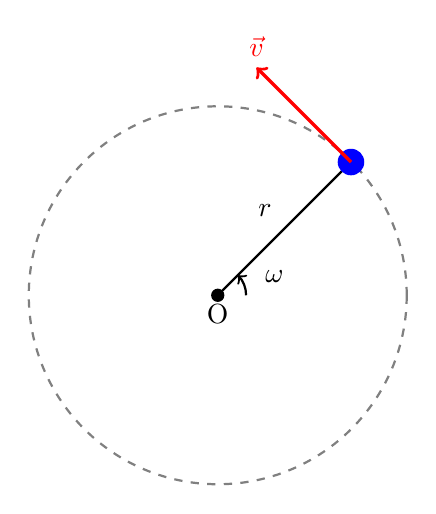
\begin{tikzpicture}[scale=1.2]
% Cercle
\draw[thick, gray, dashed] (0,0) circle (2);
% Axe
\fill (0,0) circle (2pt) node[below] {O};
% Rayon
\draw[thick] (0,0) -- (1.41,1.41);
\node at (0.5,0.9) {$r$};
% Point
\fill[blue] (1.41,1.41) circle (4pt);
% Vitesse tangentielle
\draw[very thick, red, ->] (1.41,1.41) -- (0.41,2.41) node[above] {$\vec{v}$};
% Omega
\draw[thick, ->] (0.3,0) arc (0:45:0.3);
\node at (0.6,0.2) {$\omega$};
\end{tikzpicture}
\end{center}

\begin{attention}
Plus un point est \textbf{éloigné} de l'axe de rotation, plus sa vitesse linéaire est \textbf{grande}, même si tous les points ont la même vitesse angulaire.
\end{attention}

\begin{exemple}{Vitesse en bout de pale d'hélice}{}
L'hélice d'un navire a un diamètre de $\SI{4}{m}$ et tourne à $\SI{120}{RPM}$ (tours par minute).
\begin{enumerate}[label=\alph*)]
    \item Quelle est la vitesse angulaire en rad/s?
    \item Quelle est la vitesse linéaire en bout de pale?
\end{enumerate}

\textbf{a) Vitesse angulaire :}
\[ \omega = \SI{120}{RPM} \times \frac{2\pi \text{ rad}}{\SI{1}{tour}} \times \frac{\SI{1}{min}}{\SI{60}{s}} = \SI{120}{RPM} \times \frac{2\pi}{60} \frac{\text{rad/s}}{\text{RPM}} = \SI{12,6}{rad/s} \]

\textbf{b) Vitesse en bout de pale :}

Le rayon est $r = \dfrac{d}{2} = \dfrac{\SI{4}{m}}{2} = \SI{2}{m}$.
\[ v = r\omega = \SI{2}{m} \times \SI{12,6}{rad/s} = \SI{25,1}{m/s} \]

Conversion en km/h : $v = \SI{25,1}{m/s} \times \dfrac{\SI{3,6}{km/h}}{\SI{1}{m/s}} = \SI{90}{km/h}$

Les extrémités des pales se déplacent à près de $\SI{90}{km/h}$!
\end{exemple}

\begin{pratiqueautonome}
L'hélice d'un navire a un diamètre de $\SI{5}{m}$ et tourne à $\SI{90}{RPM}$.

\begin{enumerate}[label=\alph*)]
    \item Calculez la vitesse angulaire en rad/s.
    \item Calculez la vitesse linéaire en bout de pale. Exprimez votre réponse en m/s et en km/h.
\end{enumerate}

\espaceresolution[5cm]
\reponsepratique{a) $\omega \approx \SI{9,4}{rad/s}$ \quad b) $v \approx \SI{23,6}{m/s} \approx \SI{85}{km/h}$}
\end{pratiqueautonome}

\subsection{Accélération angulaire}

\begin{definition}[title=Accélération angulaire moyenne]
L'\textbf{accélération angulaire moyenne} $\alpha$ est le taux de variation de la vitesse angulaire :
\begin{equationimportante}
\begin{equation}
\alpha_{moy} = \frac{\Delta\omega}{\Delta t}
\end{equation}
\end{equationimportante}

L'unité SI est le \textbf{radian par seconde carrée} (rad/s²).
\end{definition}

\subsubsection{Accélération tangentielle}

L'accélération tangentielle est due à la variation du \textbf{module} de la vitesse :

\begin{equationimportante}
\begin{equation}
a_t = r\alpha
\end{equation}
\end{equationimportante}

\begin{exemple}{Démarrage d'un treuil}{}
Un treuil de rayon $\SI{20}{cm}$ part du repos et atteint une vitesse de $\SI{60}{RPM}$ en $\SI{5}{s}$.
\begin{enumerate}[label=\alph*)]
    \item Quelle est son accélération angulaire?
    \item Quelle est l'accélération tangentielle du câble?
\end{enumerate}

\textbf{a) Accélération angulaire :}

Conversion de la vitesse finale :
\[ \omega_f = \SI{60}{RPM} \times \frac{2\pi}{60} \frac{\text{rad/s}}{\text{RPM}} = \SI{6,28}{rad/s} \]

Calcul de l'accélération :
\[ \alpha = \frac{\omega_f - \omega_i}{\Delta t} = \frac{\SI{6,28}{rad/s} - \SI{0}{rad/s}}{\SI{5}{s}} = \SI{1,26}{rad/s^2} \]

\textbf{b) Accélération tangentielle :}

Conversion du rayon : $r = \SI{20}{cm} = \SI{0,20}{m}$
\[ a_t = r\alpha = \SI{0,20}{m} \times \SI{1,26}{rad/s^2} = \SI{0,25}{m/s^2} \]
\end{exemple}

\subsection{Équations du mouvement circulaire uniformément accéléré}

Lorsque l'accélération angulaire $\alpha$ est \textbf{constante}, on peut utiliser des équations analogues à celles du MRUA :

\begin{equationimportante}
\textbf{Équations du mouvement circulaire uniformément accéléré}
\begin{align}
\omega_f &= \omega_i + \alpha \Delta t \\[0.3cm]
\Delta\theta &= \frac{1}{2}(\omega_i + \omega_f)\Delta t \\[0.3cm]
\Delta\theta &= \omega_i \Delta t + \frac{1}{2}\alpha(\Delta t)^2 \\[0.3cm]
\omega_f^2 &= \omega_i^2 + 2\alpha\Delta\theta
\end{align}
\end{equationimportante}

\subsection{Analogie translation-rotation}

\begin{center}
\renewcommand{\arraystretch}{1.6}
\begin{tabular}{|c|c|c|}
\hline
\rowcolor{bleuclair}
\textbf{Grandeur} & \textbf{Translation} & \textbf{Rotation} \\
\hline
Position & $x$ (m) & $\theta$ (rad) \\
\hline
Déplacement & $\Delta x$ (m) & $\Delta\theta$ (rad) \\
\hline
Vitesse & $v = \dfrac{\Delta x}{\Delta t}$ (m/s) & $\omega = \dfrac{\Delta\theta}{\Delta t}$ (rad/s) \\
\hline
Accélération & $a = \dfrac{\Delta v}{\Delta t}$ (m/s²) & $\alpha = \dfrac{\Delta\omega}{\Delta t}$ (rad/s²) \\
\hline
\hline
\multirow{4}{*}{Équations MRUA} & $v_f = v_i + a\Delta t$ & $\omega_f = \omega_i + \alpha\Delta t$ \\
\cline{2-3}
& $\Delta x = \frac{1}{2}(v_i + v_f)\Delta t$ & $\Delta\theta = \frac{1}{2}(\omega_i + \omega_f)\Delta t$ \\
\cline{2-3}
& $\Delta x = v_i\Delta t + \frac{1}{2}a(\Delta t)^2$ & $\Delta\theta = \omega_i\Delta t + \frac{1}{2}\alpha(\Delta t)^2$ \\
\cline{2-3}
& $v_f^2 = v_i^2 + 2a\Delta x$ & $\omega_f^2 = \omega_i^2 + 2\alpha\Delta\theta$ \\
\hline
\hline
\multicolumn{3}{|c|}{\textbf{Relations entre grandeurs linéaires et angulaires}} \\
\hline
\multicolumn{3}{|c|}{$s = r\theta$ \quad\quad $v = r\omega$ \quad\quad $a_t = r\alpha$} \\
\hline
\end{tabular}
\end{center}

\begin{remarque}[title=Puissance de l'analogie]
Si vous maîtrisez les équations du MRUA en translation, vous maîtrisez automatiquement celles de la rotation! Il suffit de remplacer :
\begin{itemize}
    \item $x \to \theta$
    \item $v \to \omega$
    \item $a \to \alpha$
\end{itemize}
\end{remarque}

\subsection{Applications maritimes}

\begin{exemple}{Freinage d'une hélice}{}
L'hélice d'un navire tourne à $\SI{150}{RPM}$. Lors de l'arrêt des machines, elle décélère uniformément et s'arrête après avoir effectué 20 tours.
\begin{enumerate}[label=\alph*)]
    \item Quelle est la décélération angulaire?
    \item Combien de temps dure le freinage?
\end{enumerate}

\textbf{Données :}
\begin{itemize}
    \item $\omega_i = 150 \times \frac{2\pi}{60} = \SI{15,7}{rad/s}$
    \item $\omega_f = \SI{0}{rad/s}$
    \item $\Delta\theta = 20 \times 2\pi = \SI{125,7}{rad}$
\end{itemize}

\textbf{a) Décélération angulaire :}
\begin{align*}
\omega_f^2 &= \omega_i^2 + 2\alpha\Delta\theta \\
0 &= 15,7^2 + 2\alpha(125,7) \\
\alpha &= \frac{-246,5}{251,4} = \SI{-0,98}{rad/s^2}
\end{align*}

\textbf{b) Temps de freinage :}
\[ \Delta t = \frac{\omega_f - \omega_i}{\alpha} = \frac{0 - 15,7}{-0,98} = \SI{16,0}{s} \]
\end{exemple}

\begin{exemple}{Radar rotatif}{}
Un radar de navigation effectue un balayage complet toutes les $\SI{3}{s}$.
\begin{enumerate}[label=\alph*)]
    \item Quelle est sa vitesse angulaire en rad/s et en RPM?
    \item Si l'antenne a une longueur de $\SI{1,5}{m}$, quelle est la vitesse linéaire de son extrémité?
\end{enumerate}

\textbf{a) Vitesse angulaire :}
\[ \omega = \frac{2\pi}{3} = \SI{2,09}{rad/s} = 2,09 \times \frac{60}{2\pi} = \SI{20}{RPM} \]

\textbf{b) Vitesse linéaire :}
\[ v = r\omega = 1,5 \times 2,09 = \SI{3,14}{m/s} \]
\end{exemple}

\begin{exemple}{Cabestan (exemple de calcul complet)}{}
Un cabestan de rayon $\SI{25}{cm}$ est utilisé pour haler un câble. Il démarre du repos et accélère à $\SI{0,5}{rad/s^2}$ pendant $\SI{4}{s}$, puis maintient une vitesse constante.
\begin{enumerate}[label=\alph*)]
    \item Quelle vitesse angulaire atteint-il?
    \item Combien de tours effectue-t-il pendant l'accélération?
    \item Quelle longueur de câble est halée pendant les 10 premières secondes?
\end{enumerate}

\textbf{a) Vitesse angulaire finale :}
\[ \omega_f = \omega_i + \alpha\Delta t = 0 + 0,5 \times 4 = \SI{2}{rad/s} \]

En RPM : $\omega_f = 2 \times \frac{60}{2\pi} = \SI{19,1}{RPM}$

\textbf{b) Déplacement angulaire pendant l'accélération :}
\[ \Delta\theta = \omega_i\Delta t + \frac{1}{2}\alpha(\Delta t)^2 = 0 + \frac{1}{2}(0,5)(4)^2 = \SI{4}{rad} \]

Nombre de tours : $\frac{4}{2\pi} = 0,64$ tour

\textbf{c) Longueur de câble halée en 10 s :}

Phase 1 (0 à 4 s, accélération) : $\Delta\theta_1 = \SI{4}{rad}$

Phase 2 (4 à 10 s, vitesse constante) : 
\[ \Delta\theta_2 = \omega \times \Delta t = 2 \times 6 = \SI{12}{rad} \]

Total : $\Delta\theta_{total} = 4 + 12 = \SI{16}{rad}$

Longueur de câble :
\[ s = r\Delta\theta = 0,25 \times 16 = \SI{4}{m} \]
\end{exemple}
